\subsubsection{10.01.15}
\begin{enumerate}
	
	\item Время начала и окончания собрания: 14:30 - 21:00.
	
	\item Цели собрания: 
	\begin{enumerate}
		
	  \item Изготовить и установить пластину, соединяющую вал сервопривода с осью и ведомой шестеренкой.
		
	  \item Спроектировать чертеж желоба из "оцинковки".
		
      \item Изготовить и установить провод, соединяющий сервопривод, опрокидывающий ковш, с сервоконтроллером.
		
	\end{enumerate}

	\item Проделанная работа:
	\begin{enumerate}
		
		\item Укрепляющая пластина была изготовлена и установлена на механизм опрокидывания ковша.
		\begin{figure}[H]
			\begin{minipage}[h]{0.2\linewidth}
				\center  
			\end{minipage}
			\begin{minipage}[h]{0.6\linewidth}
				\center{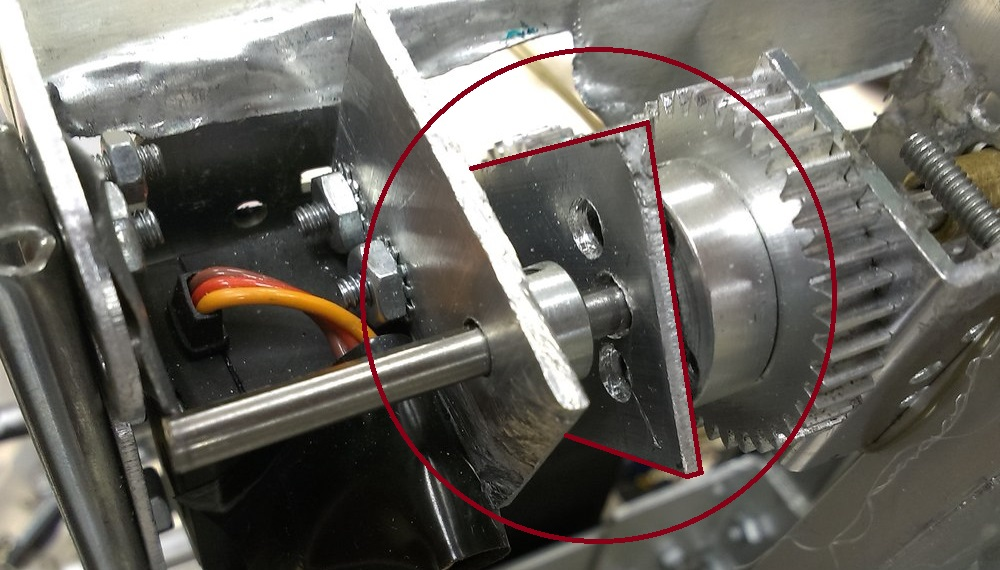
\includegraphics[scale=0.2]{days/10.01.15/images/01}}
				\caption{Укрепляющая пластина}
			\end{minipage}
		\end{figure}
		
		\item Чертеж желоба был спроектирован.
		\begin{figure}[H]
			\begin{minipage}[h]{0.2\linewidth}
				\center  
			\end{minipage}
			\begin{minipage}[h]{0.6\linewidth}
				\center{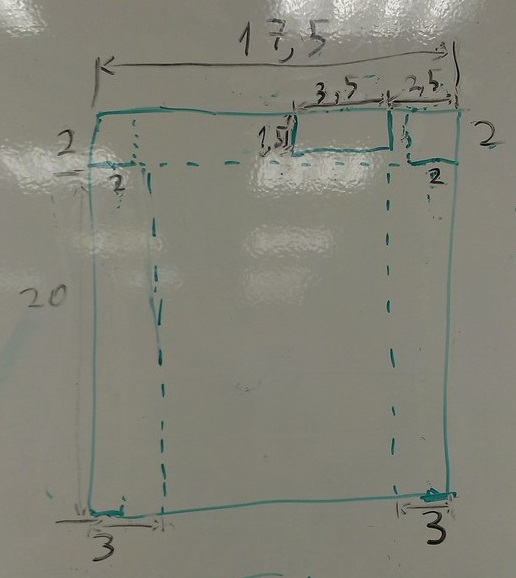
\includegraphics[scale=0.2]{days/10.01.15/images/02}}
				\caption{Чертеж развертки желоба}
			\end{minipage}
		\end{figure}
		
        \item Поскольку обычные удлиннительные провода, устанавлемые на подъемнике очень часто перебивались, для подключения сервопривода, отвечающего за опрокидывание ковша, было решено изготовить один провод повышенной прочности длиной 120-150 см. За основу был взят USB-провод с обрезанными концами, который был продет в эластичную трубку (шланг подачи воды для аквариума), которая будет защищать его от внещних воздействий. Процесс продевания провода в трубку был очень трудоемким, для этого нам понадобилась леска, которая была прикручена к проводу с одной стороны и предварительно продета в трубку (благодаря ей мы тащили провод через трубку), провод и внутренняя часть трубки были обильно смазаны жидкой смазкой для уменьшения трения. В процессе продевания было задействовано 3 человека. После продевания к концам провода были припаяны штекеры для того, чтобы провод был совместим с остальными. В конце провод был протестирован мультитестером на наличие разрывов. Таковых не оказалось.
        \begin{figure}[H]
	  	  \begin{minipage}[h]{0.24\linewidth}
	  	    \center{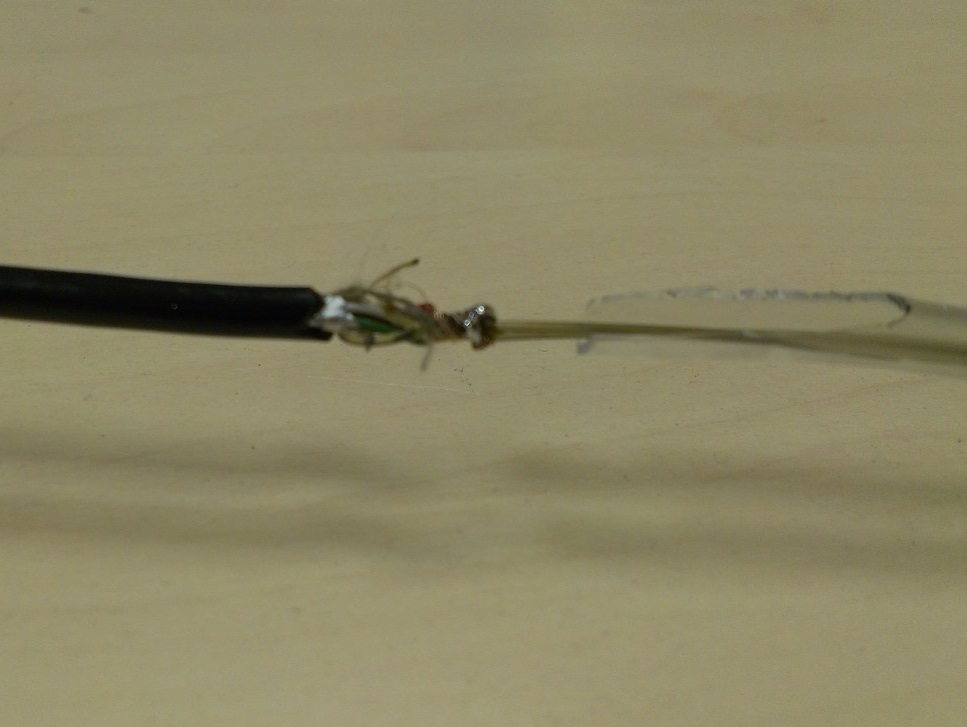
\includegraphics[scale=0.13]{days/10.01.15/images/03}}  
	  	  \end{minipage}
	  	  \hfill
	  	  \begin{minipage}[h]{0.24\linewidth}
	  		\center{
\includegraphics[scale=0.14]{days/10.01.15/images/04}}
	  	  \end{minipage}
	  	  \hfill
	  	  \begin{minipage}[h]{0.26\linewidth}
	  	  	\center{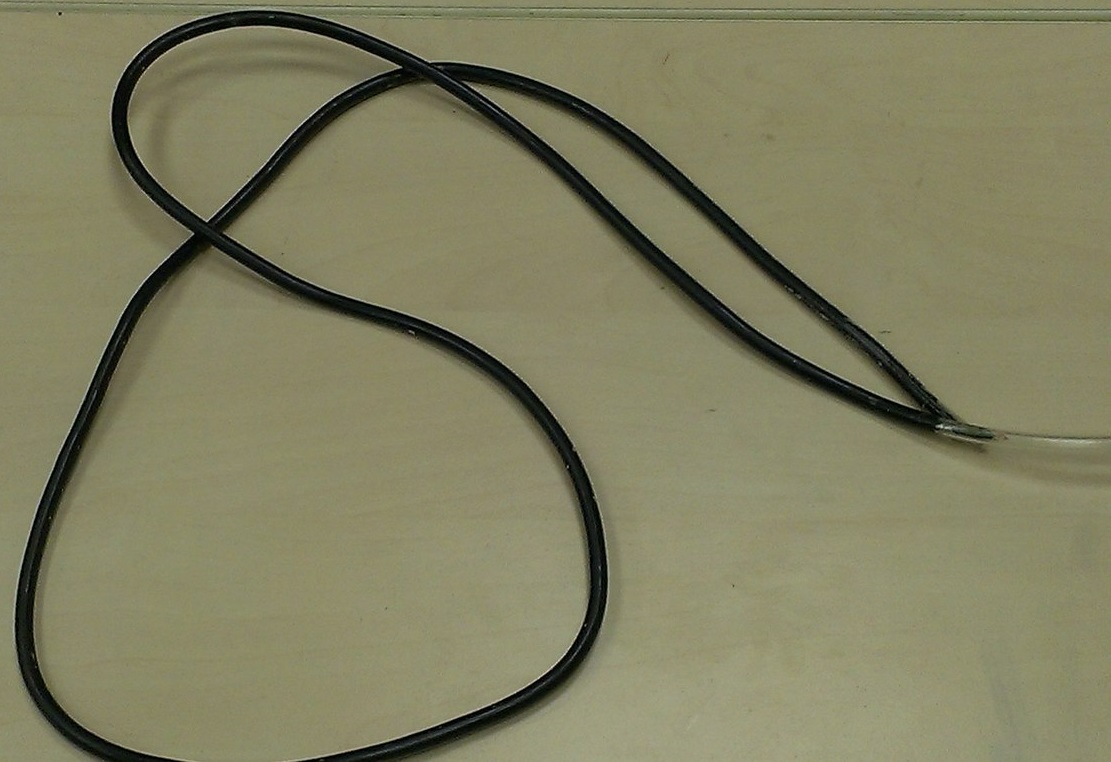
\includegraphics[scale=0.12]{days/10.01.15/images/05}} 
	  	  \end{minipage}
	  	  \hfill
	  	  \begin{minipage}[h]{0.24\linewidth}
	  	  	\center{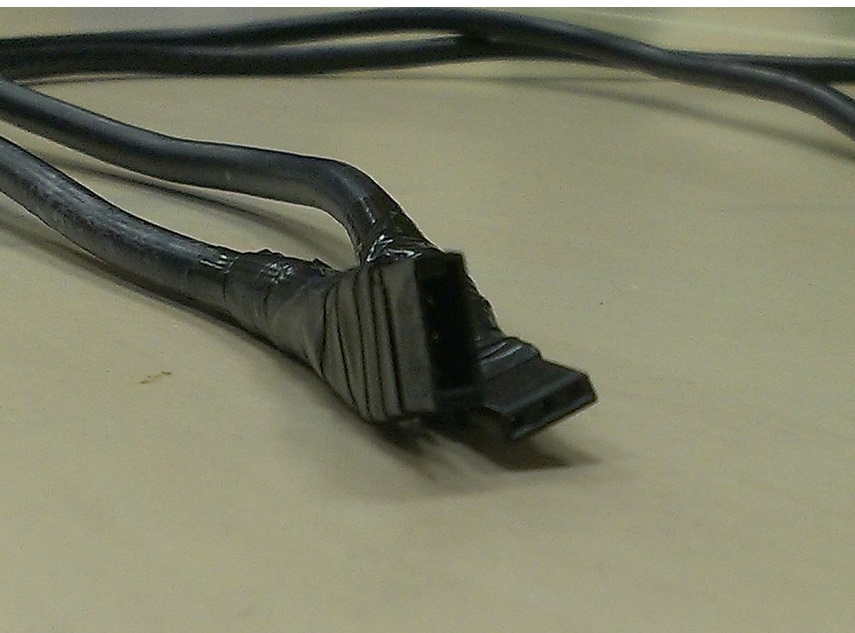
\includegraphics[scale=0.14]{days/10.01.15/images/06}}
	  	  \end{minipage}
	  	  \caption{Этапы создания провода}
	   \end{figure}

	\end{enumerate}
	
	\item Итоги собрания:
	\begin{enumerate}
		
	  \item Укрепляющая пластина установлена.
		
  	  \item Чертеж желоба готов.
		
      \item Провод для сервопривода изготовлен.
		
	\end{enumerate}
	
	\item Задачи для последующих собраний:
	\begin{enumerate}
		
	  \item Изготовить из листа стали желоб и установить его на робота.
		
	  \item Закрепить новый сверхпрочный провод на подъемнике.
			
	\end{enumerate}
\end{enumerate}
\fillpage
